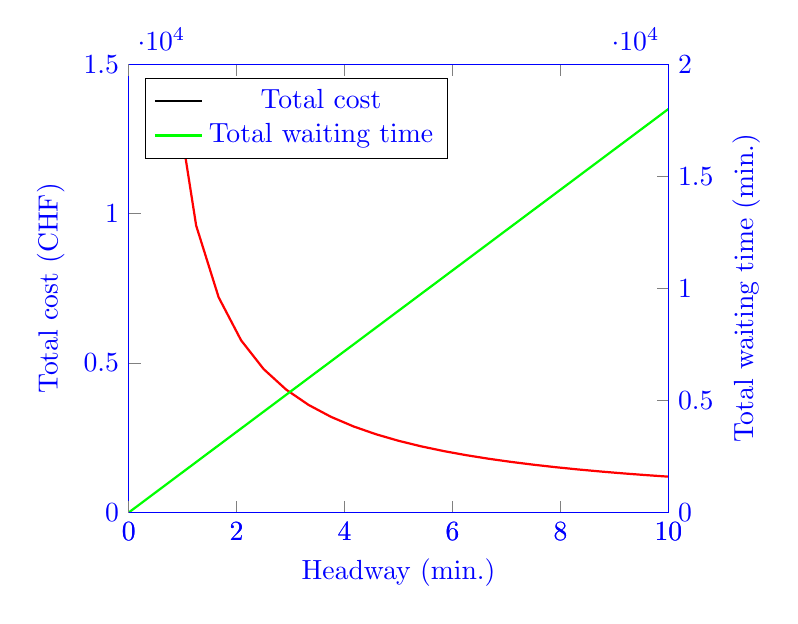
\begin{tikzpicture}[
  blue,
  declare function = {
    cost(\x) = \T * \r / \x ;
    waiting(\x) = \T * \x * \f / 2 ;
  }
]
  \def \T{60}
  \def \f{60}
  \def \r{200}
  \begin{axis}[
      xlabel={Headway (min.)},
      ylabel={Total cost (CHF)},
      axis y line* = left, % the '*' avoids arrow heads
      domain=0:10,
      xmin=0,
      xmax=10,
      ymin=0,
      ymax=15000,
      restrict y to domain=0:15000,
      axis on top,
    ]
    \addplot+[red, thick, no marks] {cost(x)}; \label{plot_cost}    
  \end{axis}
  
  \begin{axis}[
      ylabel={Total waiting time (min.)},
      axis y line* = right, % the '*' avoids arrow heads
      domain=0:10,
      xmin=0,
      xmax=10,
      ymin=0,
      ymax=20000,
      axis on top,
      legend pos=north west,
    ]
    \addlegendimage{/pgfplots/refstyle=plot_cost}\addlegendentry{Total
      cost}
    \addplot+[green, thick, no marks] {waiting(x)};
    \addlegendentry{Total waiting time}
  \end{axis}
\end{tikzpicture}
